\documentclass[journal]{IEEEtran}

\usepackage{graphicx} 
\usepackage{caption} 
\usepackage{siunitx} 
\usepackage{subcaption} 
\captionsetup[table]{skip=10pt}
\usepackage[margin=1in]{geometry} 
\usepackage{amsmath,amsthm,amssymb}
\usepackage[noend]{algpseudocode}
\usepackage{float}
\makeatletter
\def\BState{\State\hskip-\ALG@thistlm}
\makeatother

\graphicspath{{media/}}

\begin{document}

\title{Team 9 ROB 550 BotLab}

\author{Peter Mitrano, Sid Dey, Nathaniel Cox}

\maketitle

\begin{abstract}
In the Botlab lab, teams are tasked with
\end{abstract}
\IEEEpeerreviewmaketitle

\section{Introduction}
\IEEEPARstart{T}{h}e goal of the BotLab is to \dots

In this report, we discuss our implementation of SLAM, report on our systems accuracy and performance, and discuss our approach to several specific challenges like frontier exploration and the ``kidnapping'' problem.

\section{Methodology}

    Our SLAM algorithms consists of iteratively performing a localization step then a mapping step. On top of this, we choose frontier cells to explore and plan paths to those frontiers using A* on our occupancy grid.
    
    \subsection{Simultaneous Localization and Mapping (SLAM)}
    
        SLAM is a well established class of algorithms which generally involve a iterative process of building a map and localizing to that map. Figure \ref{fig:sys} shows a block diagram of how our specific SLAM implementation works. They key functions of our implementation include Bresenham's algorithm to ray trace beams and find occupied and free cells and a particle filter to estimate our pose. Within the particle filter, we used an action model based on odometry to propagate the particles, and a sensor model to weight the particles.
        
        \begin{figure}[b]
            \centering
            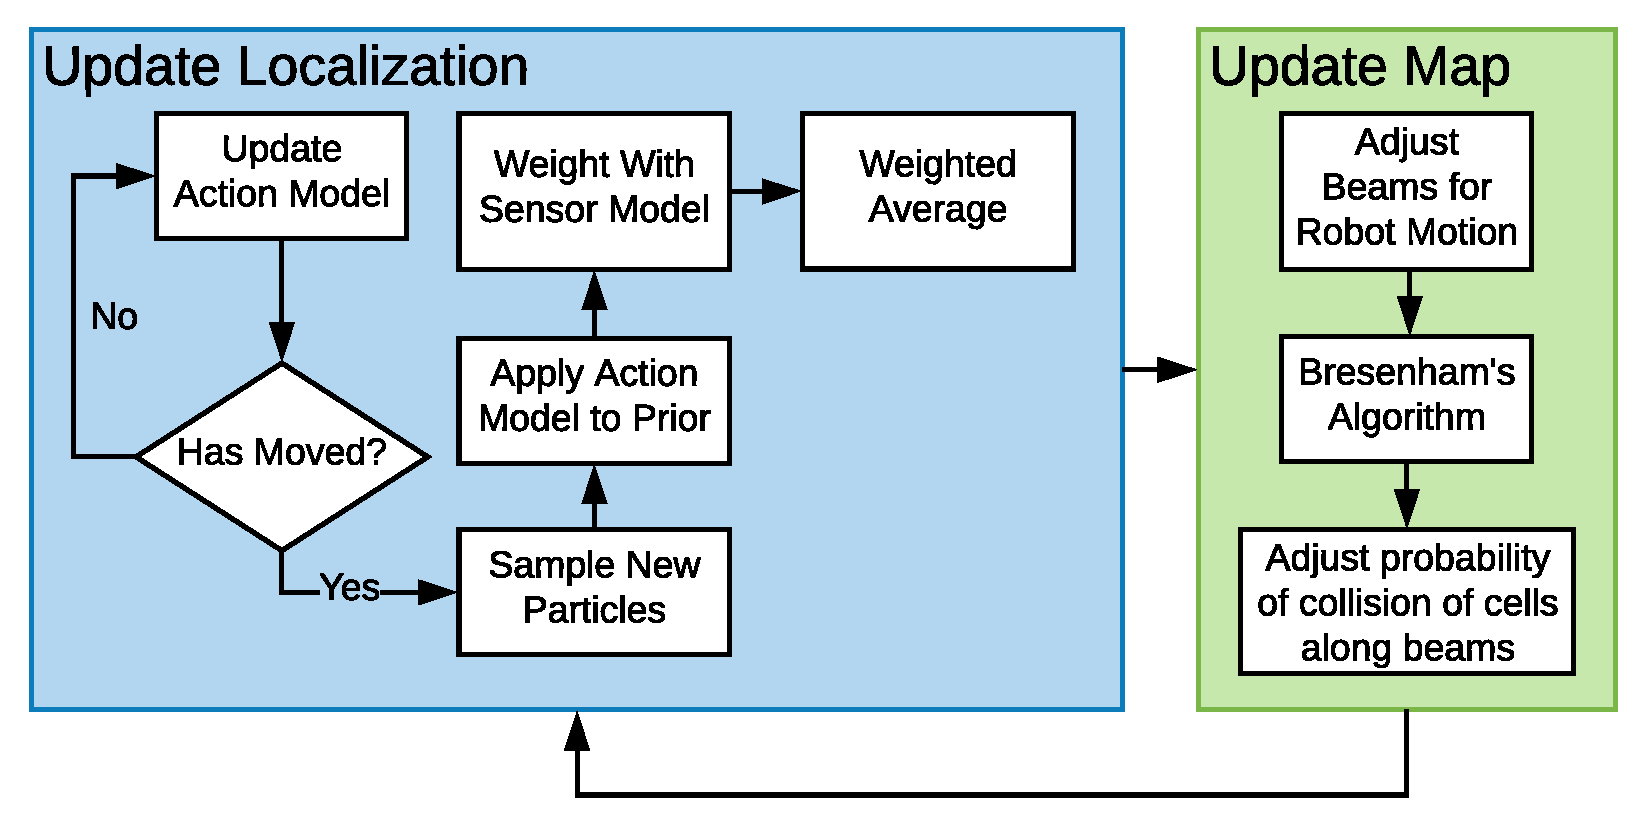
\includegraphics[width=1\linewidth]{slam.pdf}
            \caption{System diagram}
            \label{fig:sys}
        \end{figure}
    
        \subsubsection{Mapping}
        
        \subsubsection{Monte Carlo Localization}
        
        \subsubsection{Action Model}
            % Here,I shall write something just to get started...(TODO: deletemewhenyouseeme)
            
            % TODO: Describe the action model you used. 
            
            
            % TODO: Include the equations you used
            % TODO: Include a table of the values of any uncertainty parameters.  
            
            
            
            % TODO: Explain how you chose these values.
        
         \subsubsection{Sensor Model}
         
            We implemented a sensor model to produce the associated probability of correct range for the rangefinder sensor (RPLidar A2). The approximate physical model used, based on the beam model provided by Thrun, Burgard and Fox \cite{Prob_Rob}, includes three probability distributions accounting for noise of the sensor, unexpected objects near the sensor and random, unexplained measurements.
            
            The first distribution was to model the measurement noise, which was assumed to be a univariate normal distribution with the “true” range of the rangefinder based on the distance to the nearest occupied grid in the map. We found this occupied cell by discretizing the ray cast by the rangefinder into segments equal to half the cell width (\SI{2.5}{\centi\meter}) and checking the cell log-odds at each segment. If a cell contained log-odds greater than zero (indicating the cell was occupied), then we recorded the distance as $z^{*}$, the “true” distance between a particle and an object. Ray segments were terminated before the max range of the rangefinder  ($z_{max}=\SI{3.25}{\centi\meter}$). We found the probability of an individual ray with range $ z{^k}_t $ from the generated normal distribution with expected distance of $z^{*}$ and a chosen standard deviation of \SI{2.5}{\centi\meter}. We then tuned the probability by multiplying it by a constant of $k_{hit}=0.5$.
            
            We created a Poisson distribution to account for unexpectedly close obstacles by the obstacles as sensor noise. When the range was found to be less than the expected range ($z^{*}$), we used equation \ref{eq:shortprob} to find the probability of the correct range using an event rate of $\lambda_{short} = \SI{1}{\meter}$ and constant of $k_{short} =0.1$. If we found the range greater than the expected range, the probability was considered zero from the Poisson distribution.
            \begin{equation}
            	\label{eq:shortprob}
            	p_{short}(z{^k}_t |x_t,m) = k_{rand}\lambda_{short}e^{-\lambda_{short}z{^k}_t}
            \end{equation}
            Lastly, we accounted for unexplainable measurements by creating a uniform probability distribution equal to the inverse of $z_{max}$ providing a probability that the sensor reading was correct regardless of location. After calculating the probability from the assigned distribution, we tuned it by multiplying with a constant of $k_{rand}=2.0$.
            
            We summed the tuned probabilities from each of the three distributions to find the total probability of correct range per ray cast. From these probabilities of each ray cast, we calculated the log-odds and summed for the entire lidar scan to calculate the weights used for resampling in the particle filter.
            
        \subsubsection{Particle Filter}
        
        \subsection{Planning and Exploration}
        
        \begin{figure}[t]
            \centering
            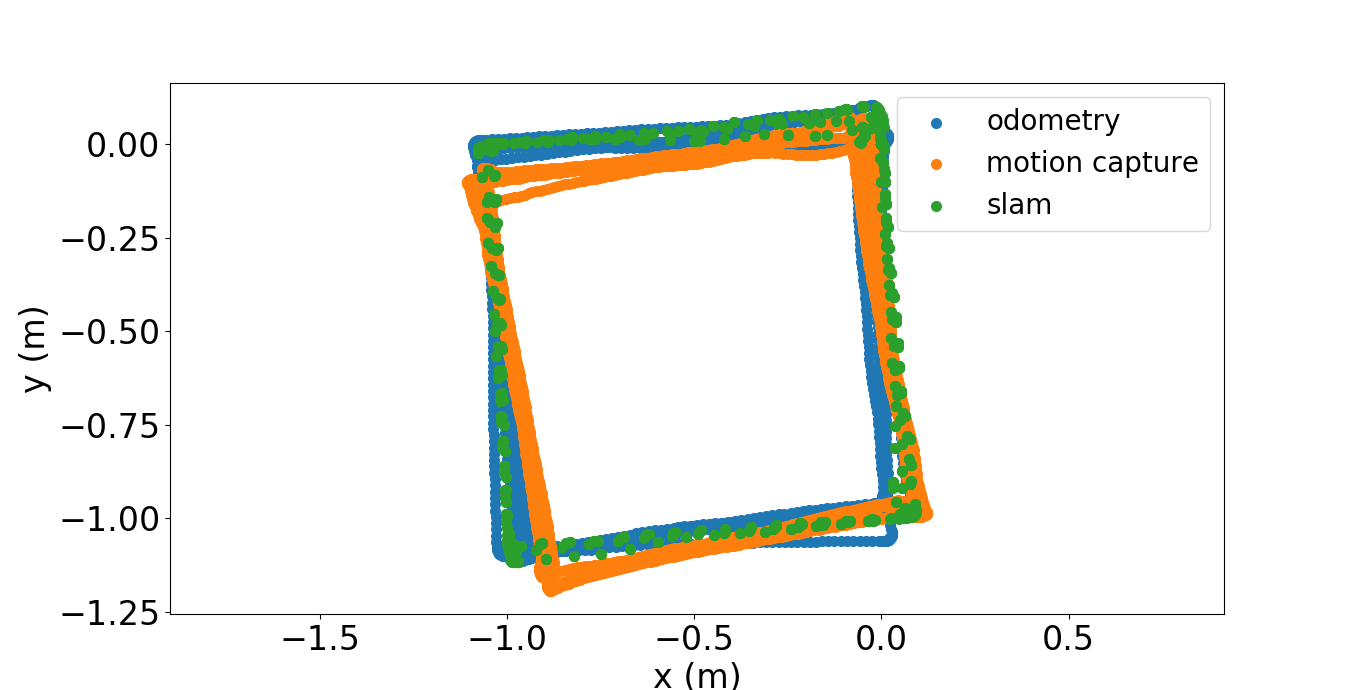
\includegraphics[width=1\linewidth]{slam_squares.png}
            \caption{SLAM Pose estimate versus motion capture pose.}
            \label{fig:slam_squares}
        \end{figure}
        
        \begin{figure}
            \centering
            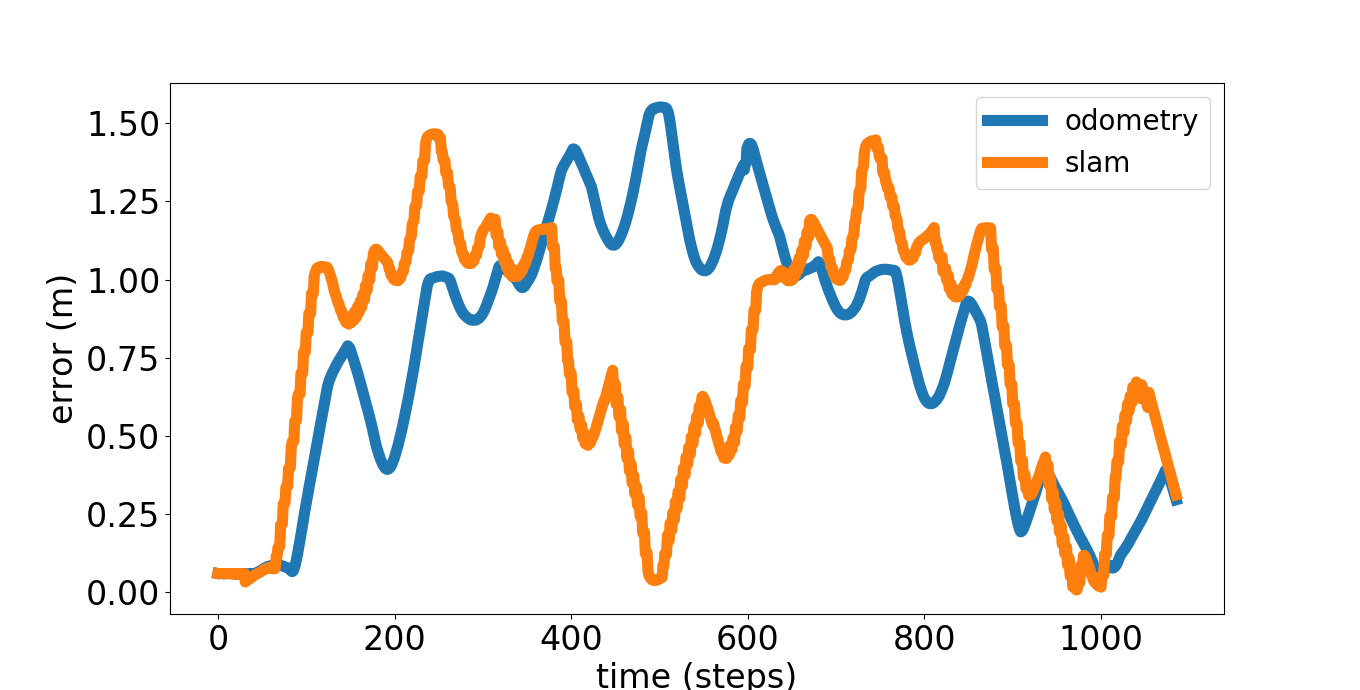
\includegraphics[width=1\linewidth]{slam_squares_error.png}
            \caption{Error over time with respect to motion capture.}
            \label{fig:slam_squares_error.}
        \end{figure}
        
        \subsubsection{Exploration}
        
        Exploring the environment to build a complete map was one of the tasks. After we build our initial map and have localized, we chose a cell near the frontier and use A* to plan a path to that cell. By iteratively choosing cells near the frontier to visit, we eventually build up a complete map of the environment.
        
        Our method for choosing which cell to explore starts with selecting the frontier whose centroid is furthest from the robots current position to explore. Next, we iterate over each cell in the frontier until we find one which is safe to navigate to. If we cannot do this, then we will continue on to search through cells in the next frontier.
        
        We discuss the successes and failures of this method in the results and discussion sections.
        
        \subsubsection{Path Planning}
        
        Our A star algorithm was able to correctly find the optimal path in all of the provided test environments. Furthermore, the mean planning time on the realistic maze scenario was \SI{2.625}{\milli\second}, which is faster then the update period of our SLAM algorithm ($\approx$\SI{100}{\milli\second}). Therefore, our planner is fast enough to operate every cycle if necessary.
        
        \begin{table}
            \centering
            \begin{tabular}{|c|c|c|c|c|c|} \hline
                & \multicolumn{5}{c|}{Planning Time (us)} \\ \hline
                Environment & min & mean & max & median & stdev \\ \hline
                convex & 194 & 197 & 218 & 195 & 7 \\ \hline
                empty & 5332 & 5630 & 6171 & 5468 & 295 \\ \hline
                maze & 2084 & 2625 & 3217 & 2533 & 410 \\ \hline
                narrow & 5404 & 136776 & 271503 & 69468 & 131305 \\ \hline
                wide & 5420 & 93529 & 268662 & 11361 & 122841 \\ \hline
            \end{tabular}
            \caption{A* Planning Times on the provided example problems. Statistics are computed on 20 trials on each map.}
            \label{tab:a_star_times}
        \end{table}
        
        \subsubsection{Motion Controller}
        
        Given our localized position and a planned path of waypoints we intend to follow, we use one of two proportional controllers to navigate along these waypoints. First, we turn to face the current target waypoint, then we follow the straight line towards that waypoint. Our controller outputs a variable forward $v$ and rotational velocity $\omega$, much like the Dubins car model. In the turning face, these control velocities are computed according to the proportional control laws \eqref{eq:turn}. We then clip the rotation velocity such that $-1 < \omega < -0.1$ or $0.1 < \omega < 1$. Here we denote the angle from the robots current pose to the target waypoint as $\phi$ and the robots current heading $\theta$. The function $d$ gives the signed smallest angle in radians between two vectors in the range $[-\pi,\pi]$. We exit the turning mode when our $d(\phi,\theta) < 0.1$.
        
        \begin{equation} \label{eq:turn}
            \begin{split}
             v &= 0 \\
             \omega &= \text{clamp}\Big[K_\text{turn}d(\phi,\theta)\Big]
            \end{split}
        \end{equation}
        
        After turning, we switch our control laws and drive towards the target waypoint. Once again, there are two cases to consider. In the case that the current waypoint is not the final waypoint in our overall plan, we move with a constant velocity of \SI{0.1}{\meter\per\second}. Otherwise, we use Equation \eqref{eq:fwd} to compute our control. The speed is clamped such that $-0.1 < v < -0.05$ or $0.05 < v < 0.1$. We discuss the decision to move at constant speed for all intermediate waypoints in the Discussion section.
        
        \begin{equation} \label{eq:fwd}
            \begin{split}
             v &=  \text{clamp}\Big[K_\text{fwd}||p, g||_2\Big] \\
             \omega &= \text{clamp}\Big[K_\text{turn2}\big(||p, g||_2+0.01\big)d(\phi,\theta)\Big]
            \end{split}
        \end{equation}
        
        The desired forward and rotational velocities and then converted to wheel speeds using Equation \eqref{eq:wheel_speeds}. Here $v_l$ is the left wheel speed in \SI{}{\radian\per\second} and $v_r$ is the right wheel speed, and $W$ is the distance between the wheels. The turning speeds and wheel speeds are controlled by a PID controller within the provided Mobilebot program. Additionally, the Mobilebot program uses a low pass filter to mitigate potential noise in velocity estimates. PID constants and filter parameters used are shown in Table \ref{tab:pid}.
        
        \begin{equation} \label{eq:wheel_speeds}
            \begin{split}
                v_l &= v - \omega\frac{W}{2} \\
                r_l &= v + \omega\frac{W}{2}
            \end{split}
        \end{equation}
        
        \begin{table}[b!]
            \centering
            \begin{tabular}{|c|c|c|c|} \hline
                kP & kI & kD & Filter Hz \\ \hline
                1.0 & 0.0 & 0.0 & 25 \\ \hline
                1.0 & 0.0 & 0.0 & 25 \\ \hline
                0.05 & 0.0 & 0.0 & 10 \\ \hline
                0.05 & 0.0 & 0.0 & 10 \\ \hline
            \end{tabular}
            \caption{PID constants used in the provided Mobilebot program}
            \label{tab:pid}
        \end{table}
    
\section{Results}

    \subsection{Simultaneous Localization and Mapping (SLAM)}
    
        \subsubsection{Mapping}
    \begin{figure}[b]
        \centering
        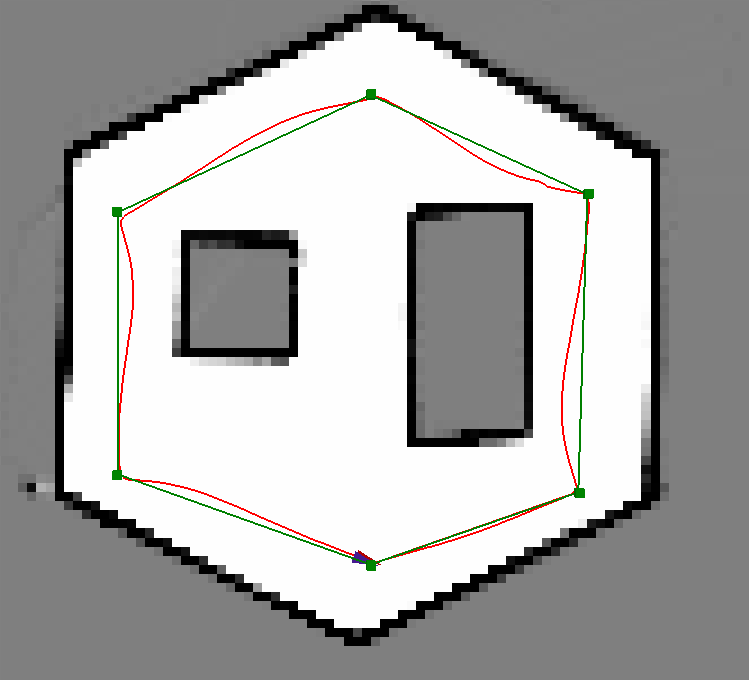
\includegraphics[width=1\linewidth]{obstacle_slam_10mx10m_5cm-map.png}
        \caption{Map built on the log file obstacle\_slam\_10mx10m\_5cm.log. True pose of the robot is shown in red.}
        \label{fig:map}
    \end{figure}
    
    \begin{figure}[b]
        \centering
        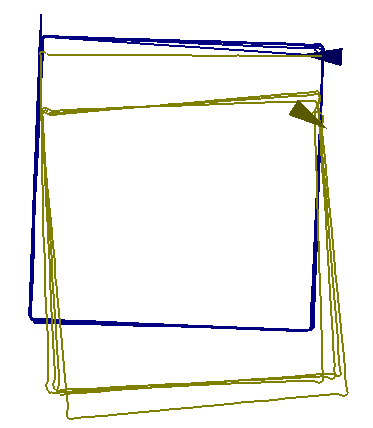
\includegraphics[width=1\linewidth]{odometry4.png}
        \caption{Plot of our robot performing four \SI{1}{\meter} squares. Blue is pose estimate from odometry, yellow is the motion capture pose.}
        \label{fig:odometry_squares}
    \end{figure}
    
        \subsubsection{Monte Carlo Localization Accuracy}
        
            Figure \ref{fig:localization} shows the robots pose over time on one of the provided log files. Here we see that the path of the robot as estimated by our localization routine is closed to the true pose as measured by motion capture. We quantified this by computing statistics of the pose error, which shows that our SLAM has an mean accuracy of \SI{4}{\centi\meter} whereas odometry has a mean accuracy of \SI{21}{\centi\meter}. We compute the distance between the true pose and point nearest in time from odometry and from SLAM, and Figure \ref{fig:localization_error} shows a plot of this error over time.
            
            \begin{figure}
                \centering
                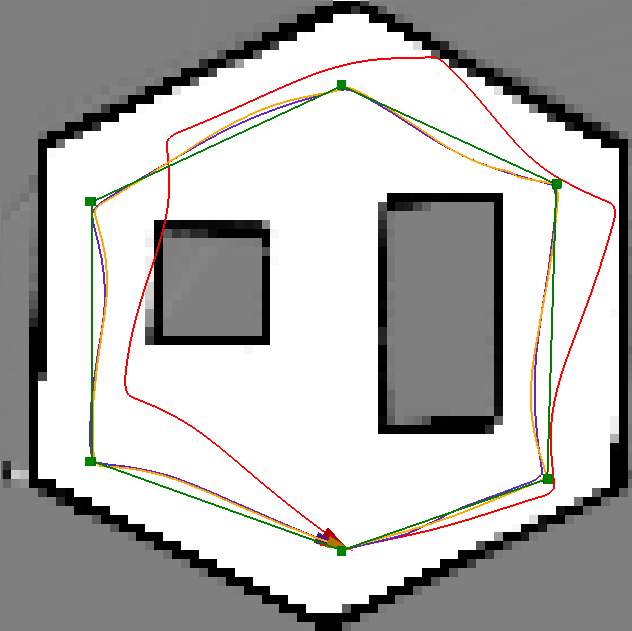
\includegraphics[width=1\linewidth]{obstacle_slam_10mx10m_5cm.png}
                \caption{Testing Localization only on obstacle\_slam\_10mx10m\_5cm.log.}
                \label{fig:localization}
            \end{figure}
            
            \begin{table}[b]
                \centering
                \begin{tabular}{|c|c|c|c|} \hline
                  & Mean (m) &   Std dev &   Max (m) \\ \hline
                  Odometry & 0.208  & 0.186  &  0.542 \\ \hline
                  SLAM & 0.039 & 0.039 &  0.217 \\ \hline
                \end{tabular}
            \caption{Statistics of the pose error for obstacle\_slam\_10mx10m\_5cm.log}
                \label{tab:localization_error}
            \end{table}
            
            \begin{figure}[t]
                \centering
                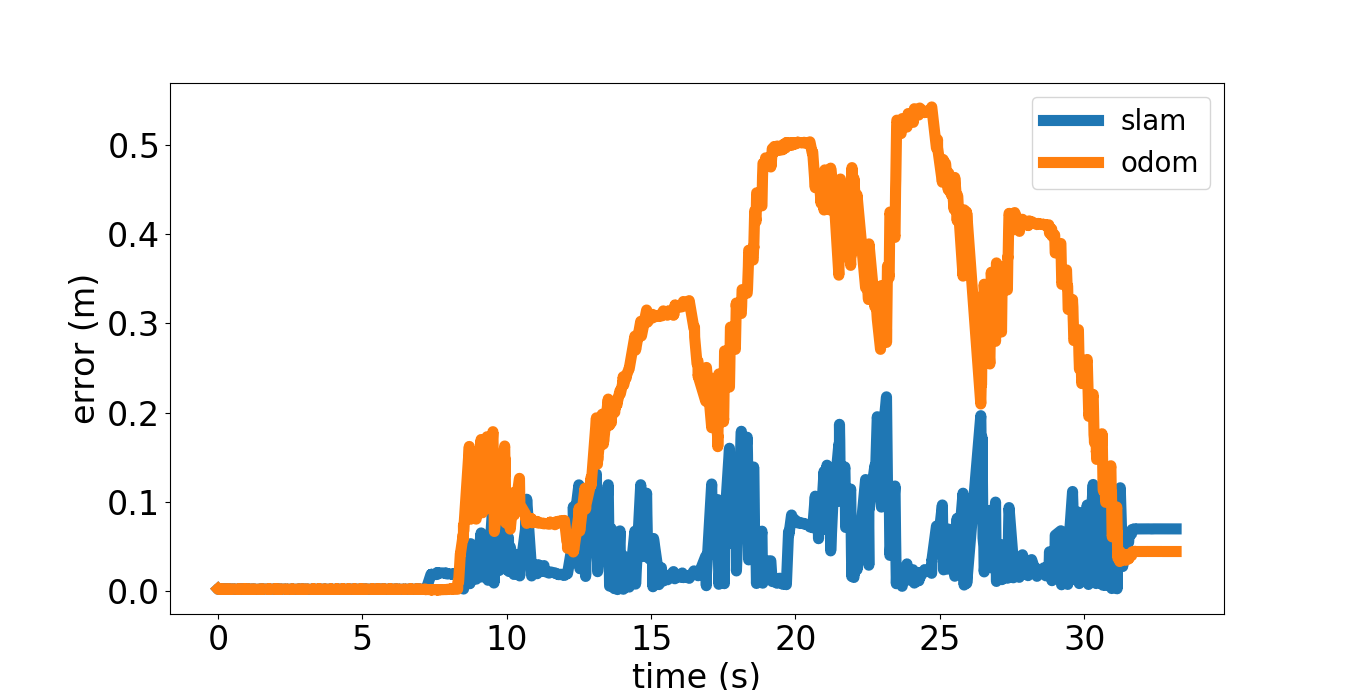
\includegraphics[width=1\linewidth]{localization_error.png}
                \caption{Error over time with respect to motion capture on the obstacle\_slam\_10mx10m\_5cm.log.}
                \label{fig:localization_error}
            \end{figure}
        
            \begin{figure}[b]
                \centering
                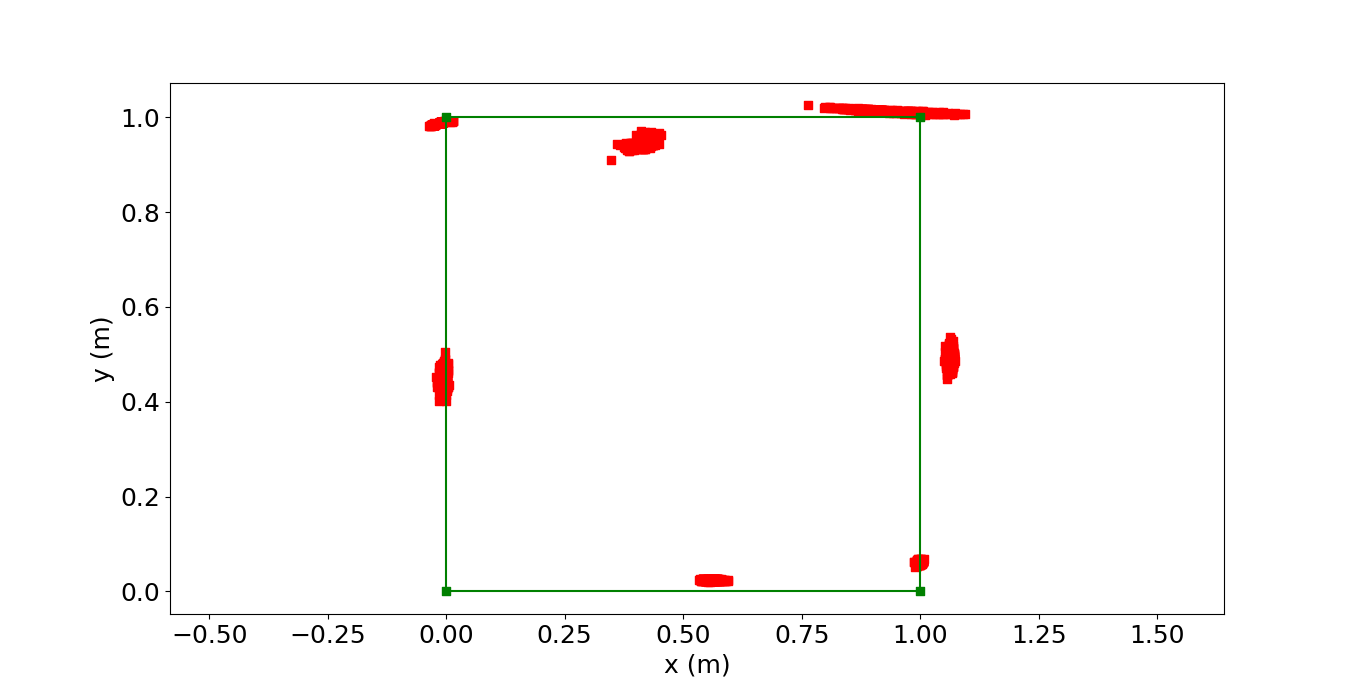
\includegraphics[width=1\linewidth]{drive_square_particles.png}
                \caption{Particles shown at various positions along a square path. Note that uncertainty is higher along the direction of motion.}
                \label{fig:square_particles}
            \end{figure}
    
        \subsubsection{Particle Filter Performance}
        
            It is essential that our SLAM system is fast enough to run in real time on our robot, otherwise the SLAM pose estimate will eventually lag behind our true pose. To quantify this, we measured how long it takes to update our paticle filter for various numbers of particles. The timing results are shown in Table \ref{tab:filter_perf}.
    
            \begin{table}[b]
                \centering
                \begin{tabular}{|c|c|} \hline
                     \# Particles & Time (ms) \\
                     100 & 28 \\ \hline
                     200 & 48 \\ \hline
                     300 & 68 \\ \hline
                     500 & 126 \\ \hline
                     1000 & 250 \\ \hline
                \end{tabular}
                \caption{Time to update the particle filter. Each time was computed as the mean of 10 updates.}
                \label{tab:filter_perf}
            \end{table}
            
            We fit a line to the data and calculated that we could handle $\approx400$ particles at \SI{10}{\hertz}.
        
            \begin{figure}[b]
                \centering
                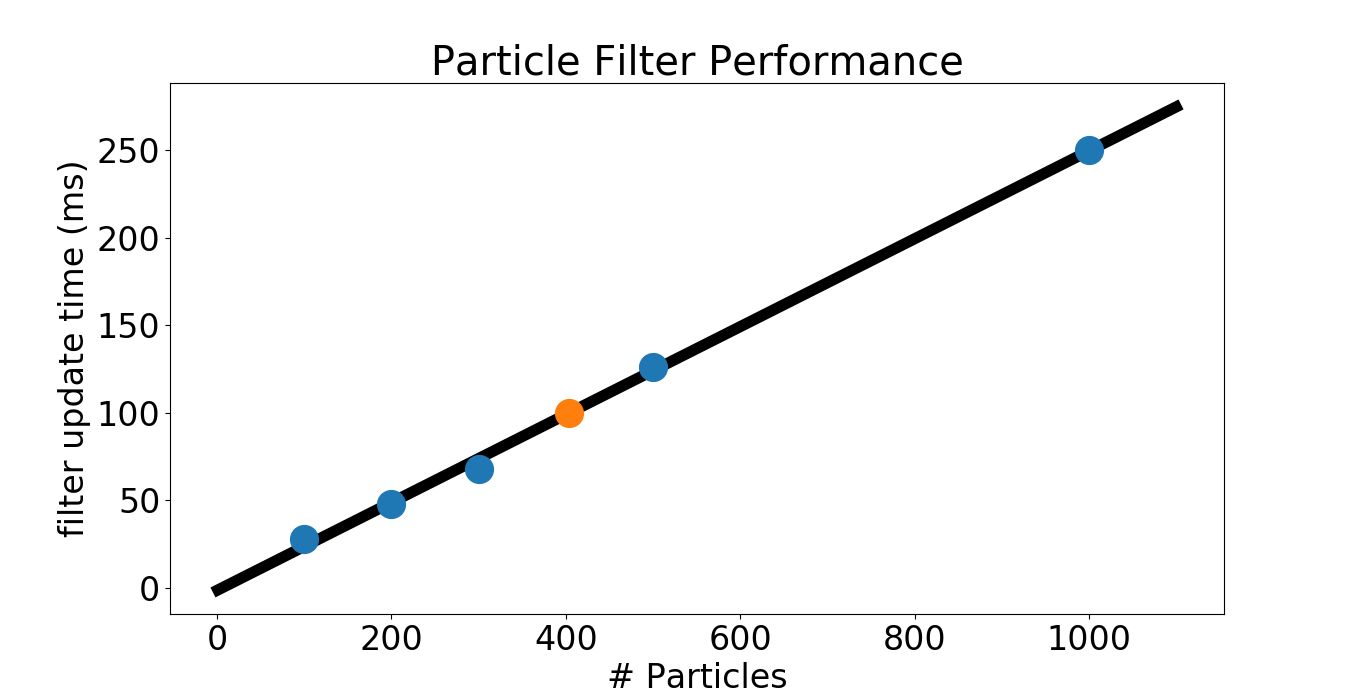
\includegraphics[width=1\linewidth]{filter_perf.png}
                \caption{Performance of the particle filter.}
                \label{fig:perf}
            \end{figure}
            
\section{Discussion}
    
    \subsection{Motion Controller}
    
    When we first used our motion controller to follow paths, we noticed that the robot spent a lot of time turning to follow waypoints that are space very close together. This meant that the robot took a long time to follow a path. To mitigate this, we both increased the position and angle tolerance for intermediate waypoints and also chose to fix the forward speed when navigating to intermediate waypoints. This way the robot did not stop, in the event that the next waypoint is in a straight line, which was often the case in our experience, that path is execute more smoothly and more quickly.

\section{Conclusion}

    Group 9 successfully completed the BotLab lab, ...

\bibliographystyle{IEEEtran}
\bibliography{550-botlab}

\newpage

\section{Appendix}

\end{document}